\begin{figure}[htbp]
    \centering
    \begin{subfigure}[b]{0.49\textwidth}
       \centering
       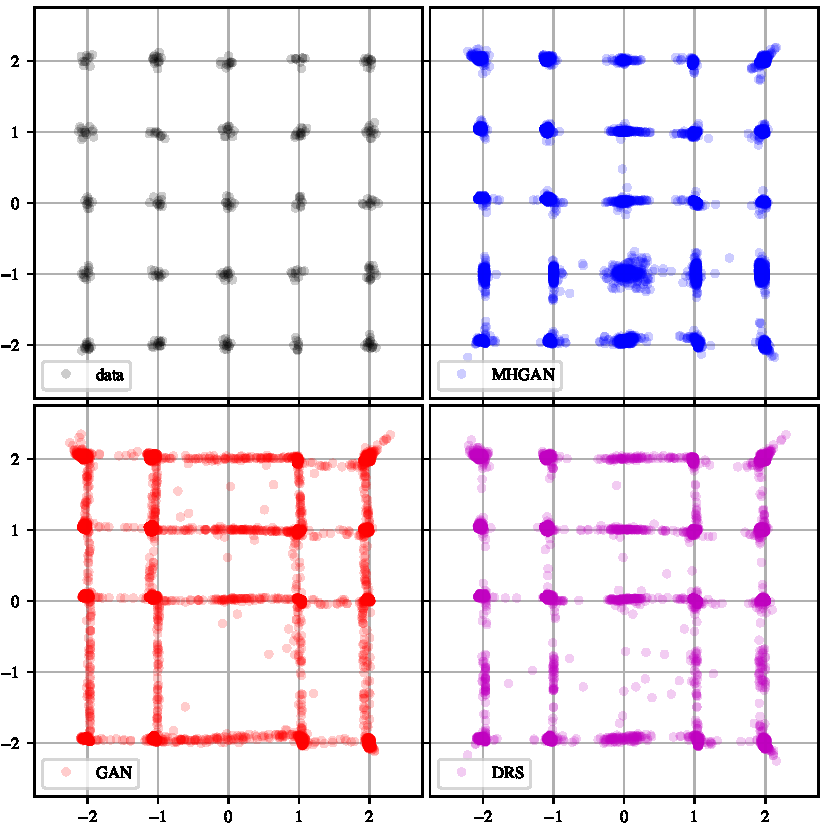
\includegraphics[scale=0.5]{figures/mog_example_30.pdf}
       \caption{epoch 30}
    \end{subfigure}
    \hfill
    \begin{subfigure}[b]{0.49\textwidth}
       \centering
       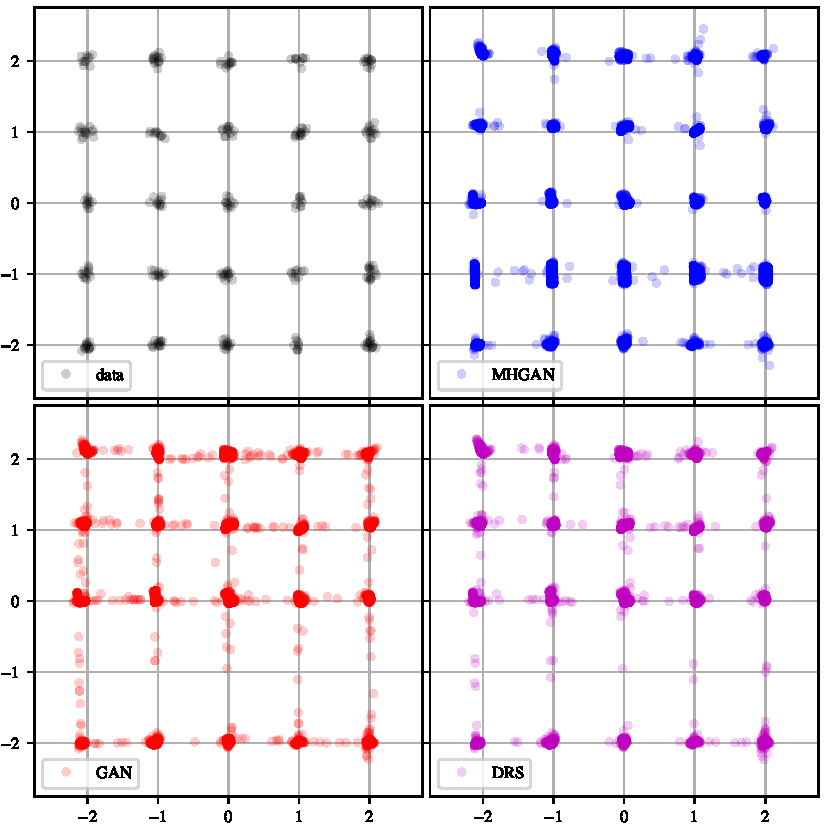
\includegraphics[scale=0.5]{figures/mog_example_150.pdf}
       \caption{epoch 150}
    \end{subfigure}
    \caption{{\small
    Data in the 25 Gaussians example (upper-left)\@.
    The other GAN setups are shown in the other figures.
    The MH-GAN corrects areas of mis-assigned mass in the original GAN\@.
    DRS appears visually closer to the original GAN than the data, whereas the MH-GAN appears closer to the actual data.
    We show the state of the generators at epoch 30 (when MH-GAN begins showing large gains) on the left and epoch 150 (the final epoch) on the right.
    }}
    \label{fig:mog_example}
\end{figure}

